
\chapter{Лораны цуваа
}
\section{Лораны цуваа} \index{Лораны цуваа}
$|z-a|<R$ дугуй дээр голоморф функцийг $z-a$-ийн сөрөг биш зэрэгтээр бичигдэх Тейлорын цуваатай өмнөх бүлэгт танилцсан. $z-a$-ийн эерэг ба сөрөг зэрэгтээр бичигдсэн
$$\sum\limits_{n=-\infty}^\infty c_n(z-a)^n$$
(энд $a$-бэхэлсэн комплекс тоо, $c_n$-тогтмол комплекс коэффициентууд) цувааг Лораны цуваа гэдэг.
\begin{thm}
\textbf{(Лоран).} \index{Лораны теорем}Цагириг хэлбэрийн 
$$V=\{z:r<|z-a|<R\}, \quad r\geq 0, \quad R\leq \infty$$
муж дээр голоморф аливаа $f(z)$ функц нийлэх
\begin{eqnarray} \label{6.1}
     f(z)=\sum\limits_{n=-\infty}^\infty c_n(z-a)^n
\end{eqnarray}
цувааны нийлбэр дүрстэй тавигдана. Коэффициентууд нь дараах томьёогоор олдоно:
\begin{eqnarray} \label{6.2}
     c_n=\frac{1}{2\pi i}\int\limits_{|z-a|=\rho} \frac{f(\zeta)d\zeta}{(\zeta -a)^{n+1}}, \quad n=0,\pm 1, \pm 2, \ldots
\end{eqnarray}
үүнд $r<\rho < R$ байна.
\begin{center}
    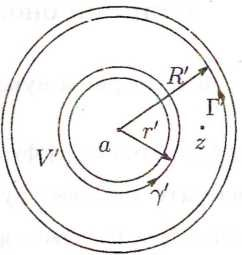
\includegraphics[width=4cm]{Zurag/20.jpg}
    \captionof{figure}{}
        \label{}
\end{center}
\end{thm}
\begin{prf}
Бэхлэн авсан $z$ цэг дотор нь байхаар $V'\Subset V$ гэсэн шинэ цагираг муж байгуулъя: $V'=\{\zeta :r'<|\zeta-a|<R'\}$ энд $r<r'$, $R'<R$. Кошийн интеграл томьёо ёсоор
\begin{eqnarray} \label{6.3}
     f(z)=\frac{1}{2\pi i} \int\limits_{\partial V'} \frac{f(\zeta)d\zeta}{(\zeta -z)}= \frac{1}{2\pi i} \int\limits_{\Gamma'} \frac{f(\zeta)d\zeta}{(\zeta -a)}-\frac{1}{2\pi i} \int\limits_{\gamma'} \frac{f(\zeta)d\zeta}{(\zeta -a)}
\end{eqnarray}
энд $\Gamma '=\{|\zeta -a|=R'\}$ ба $\gamma '=\{|\zeta -a|=r'\}, \quad \zeta\in \Gamma '$ байх үед $\left|\dfrac{z-a}{\zeta -z}\right|=q<1$ тул 
$$\frac{1}{\zeta-z}=\frac{1}{(\zeta -z)\left(1-\frac{z-a}{\zeta -a}\right)}=\sum\limits_{n=0}^\infty \frac{(z-a)^n}{(\zeta -a)^{n+1}}$$
$\zeta \in \Gamma'$-ээрээ абсолют бөгөөд жигд нийлнэ. Үүнийг зааглагдсан $\dfrac{1}{2\pi i}f(\zeta)$ функцээр үржүүлж (жигд нийлэлт алдагдахгүй тул) дараа нь $\Gamma '$ тойргоор гишүүнчлэн интегралчлавал
\begin{eqnarray} \label{6.4}
    \frac{1}{2\pi i}\int\limits_{\Gamma'} \frac{f(\zeta)d\zeta}{(\zeta -z)}= \sum\limits_{n=-\infty}^\infty c_n(z-a)^n
\end{eqnarray}
\begin{eqnarray} \label{6.5}
    c_n=\frac{1}{2\pi i}\int\limits_{\Gamma'} \frac{f(\zeta)d\zeta}{(\zeta -a)^{n+1}}, \quad (n=0,1,\ldots)
\end{eqnarray}
(\ref{6.3}) томьёоны хоёрдох интеграл арай өөрөөр задлагдана. $\zeta \in \gamma'$ байх үед $\left|\dfrac{z-a}{\zeta -z}\right| =q<1$ тул бид $\gamma'$ дээр абсолют бөгөөд жигд нийлэх геометр прогрессыг 
$$-\frac{1}{\zeta -z}=\frac{1}{(\zeta -a)\left(1-\frac{\zeta -a}{z-a}\right)}=\sum\limits_{n=1}^\infty \frac{(\zeta-a)^{n-1}}{(z -a)^{n}}$$
байдалтай гарган авна. Үүнийг мөн л зааглагдсан $\dfrac{1}{2\pi i}f(\zeta)$
функцээр үржүүлж $\gamma '$-ээр гишүүнчлэн интегралчилбал
\begin{eqnarray} \label{6.6}
    -\frac{1}{2\pi i}\int\limits_{\gamma'} \frac{f(\zeta) d\zeta}{\zeta -z}=\sum\limits_{n=1}^\infty \frac{d_n}{(z-a)^n},
\end{eqnarray}
энд 
\begin{eqnarray} \label{6.7}
    d_n= \frac{1}{2\pi i}\int\limits_{\gamma'} f(\zeta)(\zeta -z)^{n-1}d\zeta, \quad (n=1,2,\ldots)
\end{eqnarray}
(\ref{6.7}) ба (\ref{6.5}) томьёонуудаас
\begin{eqnarray}
    c_n=d_{-n}= \frac{1}{2\pi i}\int\limits_{\gamma'} f(\zeta)(\zeta -z)^{-n-1}d\zeta, \quad (n=-1,-2, \ldots)
\end{eqnarray}
болж (\ref{6.6})
\begin{equation}
    \tag{6.6'} \label{6.6'}
    -\frac{1}{2\pi i}\int\limits_{\gamma'} \frac{f(\zeta)d\zeta}{(\zeta -a)}=\sum\limits_{n=-1}^{-\infty} c_n(z-a)^n
\end{equation}
(\ref{6.4}) ба (\ref{6.6'})-ийг (\ref{6.3}) тавибал (\ref{6.1}) задаргаа гарна. Кошийн интеграл томьёо ёсоор $\Gamma'$ ба $\gamma '$ тойргуудыг тэдэнтэй гомотоп дурын тойргоор (тухайлбал $|\zeta -a|=\rho, \quad r<\rho <R$.) сольж болох тул (\ref{6.2}) томьёо гарна.
 \end{prf}
\begin{dfn}
Коэффициентууд нь (\ref{6.2}) томьёонуудаар тодорхойлогдох (\ref{6.1}) цувааг цагираг $V$ муж дахь $f(z)$ функцийн Лораны цуваа гэнэ. Энэ цувааны сөрөг биш зэрэгтээр тавигдсан хэсгийг зөв хэсэг, сөрөг зэрэгтээр тавигдсан хэсгийг гол хэсэг \index{Лораны цувааны гол ба зөв хэсэг} гэж нэрлэнэ. Иймд
\begin{eqnarray}
    \sum\limits_{n=-\infty}^\infty c_n(z-a)^ n
\end{eqnarray}
цуваа
\begin{eqnarray}
    S_1=\sum\limits_{0}^\infty c_n(z-a)^n \quad \text{ба} \quad S_2=\sum\limits_{n=-1}^{-\infty} c_n(z-a)^ n
\end{eqnarray}
цуваануудын нийлбэр байдлаар тодорхойлогдоно. \\
$S_1$ цуваа нь ердийн зэрэгт цуваа тул түүний нийлэлтийн радиус $R$
\begin{eqnarray}
    \frac{1}{R}=\overline{\lim\limits_{n\rightarrow \infty}} \sqrt[n]{|c_n|}
\end{eqnarray}
томьёогоор $S_2$ цувааны нийлэлтийн радиус $r$
\begin{eqnarray}
    r=\overline{\lim\limits_{n\rightarrow \infty}} \sqrt[n]{|c_{-n}|}
\end{eqnarray}
томьёогоор тус тус тогтоогдохыг төвөггүй харуулж болно. $R>r$ байж болохгүй. Учир нь тийм байвал цувааны нийлэх муж хоосон олонлог байхад хүрнэ.

Абелийн теорем ёсоор $V$ цагираг мужид компактаар орших аливаа дэд олонлог дээр жигд нийлэх тул Вейерштрассын теорем ёсоор түүний нийлбэр $V$ дээр голоморф байна. Эдгээр тэмдэглэл дээр тулгуурлан Лораны цувааны задаргааны цор ганц байхыг тогтоож болно.
\end{dfn}
\begin{thm} \label{Теорем 6.2}
Функцийн Лораны задаргаа цор ганц \index{Лораны задаргааны цор ганц}, өөрөөр хэлбэл $f(z)$ функц $0\leq r<|z-a|<R$ цагираг дээр 
\begin{eqnarray} \label{6.13}
    f(z)=\sum\limits_{k=-\infty}^\infty a_n(z-a)^ k
\end{eqnarray}
дүрстэй цуваанд задарсан бол $a_k$ коэффициентууд (\ref{6.5}) томьёогоор илэрхийлэгдэнэ.
\end{thm}
\begin{prf}
$\gamma =|z-a|=\rho$ тойрог авъя. (\ref{6.13})-ын хоёр талыг 
$\dfrac{1}{2\pi i}(z-a)^{-n-1}, \quad (n=-1,-2,\ldots)$-ээр үржүүлж $\gamma$ тойргоор гишүүнчлэн интегралчилбал 
$$\sum\limits_{n=-\infty}^\infty a_n \int\limits_\gamma (z-a)^{k-n-1}dz= \int\limits_\gamma \frac{f(z)dz}{(z-a)^{n+1}}$$
бөгөөд зэргийн ортогональ чанараар $k\neq n$ байх бүх интеграл тэг болж $k=n$ тохиолдолд $2\pi i$ болох тул
$$2\pi i a_n=\int\limits_\gamma  \frac{f(z)dz}{(z-a)^{n+1}}, \quad (n=0, \pm 1, \ldots)$$ эндээс $c_n\equiv a_n$ болов. 
 \end{prf}
Теорем 6.2-ыг өөрөөр томьёолбол $z-a$-ийн эерэг, сөрөг зэрэгтээр задарсан нийлэх аливаа цуваа нь өөрийн нийлбэрийнхээ Лораны цуваа байна.

Лораны цувааны коэффициентуудыг (\ref{6.2}) томьёогоор бодох нь нэн ховор. Учир нь интегралчлах ажиллагаа шаардагдана. Задаргаа цор ганц байх теоремын үндсэн дээр хуулийн хүчинтэй аливаа арга хэрэглэнэ. Ийм арга бүхэн хүсэн хүлээсэн ганц л үр дүнд хүргэнэ.
\begin{exm}
$f(z)=\dfrac{1}{(z-1)(z-2)}$ функцийг $z$-ийн зэрэгтээр Лораны цуваанд задал.
\end{exm}
\begin{sol}
Энэ функц $z=1$, $z=2$ цэгүүд дээр голоморф чанараа алдана. Иймд 
$$D_1:|z|<1, \quad D_2:1<|z|<2, \quad D_3:2<|z|<\infty$$ цагирагууд дээр голоморф функц юм. $f(z)=\dfrac{1}{z-2}-\dfrac{1}{z-1}$ дүрстэй тавигдах тул 
$$\frac{1}{z-2}=-\frac{1}{2}\cdot \frac{1}{1-\frac{z}{2}}=-\frac{1}{2}\sum\limits_{n=0}^\infty \left(\frac{z}{2}\right)^n \quad (|z|<2)$$
$-\dfrac{1}{z-1}=\sum\limits_{n=0}^\infty z^n \qquad (|z|<1).$ Иймд $|z|<1$ байхад 
$$f(z)=\sum\limits_{n=0}^\infty \left(1-\frac{1}{2^{n+1}}\right) z^n \qquad \text{(Энэ нь Тейлорын цуваа)}$$
Одоо $D_2$ цагирагт
$$-\frac{1}{z-1}=-\frac{1}{z}\frac{1}{1-\frac{1}{z}}=-\frac{1}{z}\sum\limits_{n=0}^\infty \frac{1}{z-n}=-\sum\limits_{n=0}^\infty \frac{1}{z^n+1}\quad (1<|z|)$$
Иймд $1<|z|<2$ байхад 
$$f(z)=-\sum\limits_{n=-1}^{-\infty} z_n-\sum\limits_{n=0}^\infty \frac{z^n}{2^{n+1}}.$$
Одоо $D_3$ цагирагт
$$\frac{1}{z-2}=\frac{1}{z}\frac{1}{1-\frac{2}{z}}=\frac{1}{z}\sum\limits_{n=0}^\infty \left(\frac{2}{z}\right)^n=\sum\limits_{n=1}^\infty \frac{2^{n-1}}{z^n}\quad (2<|z|).$$
Иймд $2<|z|<\infty$ байхад 
$$f(z)=\sum\limits_{n=2}^\infty (2^{n-1}-1)z^{-n}.$$
\end{sol}
\begin{exm}
$f(z)=\dfrac{1}{z(1-z)}$ функцийг $z=0$, $z=1$, $z=\infty$ цэгийн орчинд Лораны цуваанд задал.  
\begin{center}
    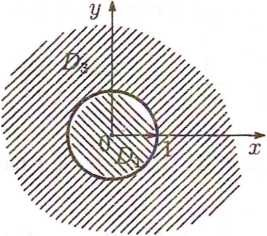
\includegraphics[width=4cm]{Zurag/21.jpg}
    \captionof{figure}{}
        \label{}
\end{center}
\end{exm}
\begin{sol}
$z=0$ ба $z=1$ нь $\dfrac{1}{z(1-z)}=\dfrac{1}{z}+\dfrac{1}{1-z}$ функцийн голоморф алдагдах цэгүүд. \\
$D_1:z=0$ цэгийн цоорхойт орчин тул $0<|z|<1$ бөгөөд 
$$\frac{1}{z(1-z)}=\frac{1}{z}+\frac{1}{1-z}=\frac{1}{z}+\sum\limits_{n=0}^\infty z^n$$ болж задаргаа гол хэсэгтээ ганц гишүүнтэй байна. \\
$D_3:z=\infty$ цэгийн орчин $1<|z|$ 
\begin{center}
    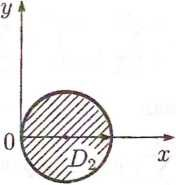
\includegraphics[width=3cm]{Zurag/22.jpg}
    \captionof{figure}{}
        \label{}
\end{center}
$$\frac{1}{z(1-z)}=-\frac{1}{z^2}\frac{1}{1-\frac{1}{z}}=-\sum\limits_{n=2}^\infty \frac{1}{z^n} \quad \left(\left|\frac{1}{z}\right|<1 \ \ \text{тул} \right)$$ 
$D_2:z=1$ цэгийн орчин $|z-1|<1$ 
$$\frac{1}{z(1-z)}=-\frac{1}{z-1}+\frac{1}{z-1+1}=-\frac{1}{z-1}+\sum\limits_{n=0}^\infty (-1)^n (z-1)^n.$$ \end{sol}
Лораны цувааны коэффициентын (\ref{6.2}) томьёо $n\geq 0$ үед Тейлорын цувааны коэффициент олох интеграл томьёотой тохирно.

$f(z)$ функц $V=\{r<|z-a|<R\}$ цагираг дээр голоморф, $\gamma =\{|z-a|=\rho\}, \quad r<\rho <R$ тойрог дээр $|f(z)|<M$ байвал задаргаа коэффициент
\begin{eqnarray} \label{6.14}
    |c_n|<\frac{M}{\rho^n},\quad n=0, \pm 1,\ldots
\end{eqnarray}
(\ref{6.14})-ийг Лораны цувааны Кошийн тэнцэл биш \index{Лораны цувааны Кошийн тэнцэл биш} гэнэ.

Одоо Лораны цуваа, Фурьегийн цуваатай хэрхэн холбогдохыг \index{Лораны цуваа, Фурьегийн цуваатай холбогдох нь} авч үзье. $[0,2\pi]\subset \mathbb{R}$ дээр интегралчилагдах $\varphi (z)$ функц Фурьегийн цуваагаар 
\begin{eqnarray}
    \varphi(t)=\frac{a_0}{2}+\sum\limits_{n=1}^\infty (a_n\cos nt +b\sin nt),
\end{eqnarray}
гэж тодорхойлогдоно. Энд
\begin{eqnarray}
\begin{split}
     &a_n=\frac{1}{\pi} \int\limits_0^{2\pi} \varphi(t)\cos nt dt \quad n=0,1,\ldots\\
    &b_n= \frac{1}{\pi} \int\limits_0^{2\pi} \varphi(t)\sin nt dt, \quad n=0,1,\ldots
\end{split}
\end{eqnarray}
Энэ цувааг Эйлерийн $\cos nt =\dfrac{e^{int}+e^{-int}}{2}$, $\sin nt =\dfrac{e^{int}-e^{-int}}{2}$ томьёо ашиглах замаар комплекс хэлбэртэй бичиж болно:
$$\frac{a_0}{2}+\sum\limits_{n=1}^\infty \left(\frac{a_n-ib_n}{2} e^{int}+\frac{a_n+ib_n}{2}e^{-int}\right) =\sum\limits_{n=-\infty}^\infty c_ne^{int}$$
энд $$c_n=\frac{a_n-ib_n}{2}=\dfrac{1}{2\pi }\int\limits_{0}^{2 \pi}\varphi (t)e^{-int}dt, \quad n=0,1,\ldots$$
$$c_n=\frac{a_{-n}+ib_n}{2}=\dfrac{1}{2\pi }\int\limits_{0}^{2 \pi}\varphi (t)e^{-int}dt, \quad n=-1,-2,\ldots$$
байна.

Коэффициентууд нь
\begin{eqnarray}
c_n=\dfrac{1}{2\pi }\int\limits_{0}^{2 \pi}\varphi (t)e^{int}dt
\end{eqnarray}
томьёонуудаар олдох
\begin{eqnarray} \label{6.18}
\sum\limits_{n=-\infty}^\infty c_ne^{int}
\end{eqnarray}
цуваа $\varphi$ функцийн комплекс хэлбэртэй тавигдсан Фурьегийн цуваа байна.

$e^{int}=z$ ба $\varphi (t)=f(e^{it})=f(z)$ гэж авбал \ref{6.18} цуваа 
\begin{eqnarray} 
\sum\limits_{n=-\infty}^\infty c_n z^n
\end{eqnarray}
болж коэффициентууд нь 
\begin{eqnarray}
c_n=\dfrac{1}{2\pi }\int\limits_{0}^{2 \pi} f (e^{it})e^{-int}dt= \dfrac{1}{2\pi i}\int\limits_{|z|=1} f(z)\frac{dz}{z^{n+1}}
\end{eqnarray}
Иймд $\varphi (t)$, $t\in [0, 2\pi]$ функцийн комплекс хэлбэртэй бичигдсэн Фурьегийн цуваа нь $f(z)=\varphi (t)$, $z=e^{it}$ функцийн нэгж тойрог $(|z|=1)$ дээр тавигдсан Лораны цуваа юм.

Фурьегийн цуваа $[0,2\pi]$ хэрчмийн цэг бүр дээр $\varphi (t)$-рүү нийлэх тохиолдолд ч харгалзах Лораны цувааны хувьд $R=r=1$ болж нийлэлтийн муж нь хоосон олонлог болно.

$\varphi (t)$ функц нэлээд хатуу шаардлага хангах нөхцөлд харгалзах Лораны цуваа нийлэлтийн хоосон биш мужтай байдаг.
\section{Тусгаарлагдсан онцгой цэгүүд,\\
тэдгээрийг ангилах нь
}
\begin{dfn}
$a\in\overline{\mathbb{C}}$ цэг $f(z)$ функцийн онцгой цэг, харин түүний цоорхойт ($a$-төгсгөлтэй бол $0<|z-a|<r$, $a=\infty$ бол $R<|z|<\infty)$ орчинд уул функц голоморф байвал $a$-цэгийг тусгаарлагдсан онцгой цэг \index{Тусгаарлагдсан онцгой цэг} гэнэ.

Тийм цэг рүү дөхөхөд $f(z)$ функцийн төрх ямар байхаас хамаарч тусгаарлагдсан онцгой цэгийг гурав ангилна. 
\end{dfn}
\begin{dfn}
Тусгаарлагдсан онцгой $a$ цэгийн хувьд
\begin{enumerate}
    \item [I.] $\lim\limits_{z\rightarrow a} f(z)=A$-төгсгөлтэй байвал $a$-засагдах онцгой цэг. \index{Засагдах онцгой цэг}
    \item [II.] $\lim\limits_{z\rightarrow a} f(z)=\infty$ байвал $a$-туйл.
     \item [III.] $\exists f(z)$ нь $z\rightarrow a$ үед төгсгөлтэй ч, төгсгөлгүй ч хязгаар байхгүй байвал $a$-гоц онцгой цэг гэж нэрлэнэ.
\end{enumerate}

Тусгаарлагдсан онцгой а цэгийн төрх нь түүний цоорхойт орчинд задалсан Лораны цуваатай нягт холбоотой байдаг. Төгсгөлтэй а цэгийн хувьд энэ холбоог харуулсан дараах гурван теоремтой танилцъя:
\end{dfn}
\begin{thm}
Тусгаарлагдсан онцгой $a\in\mathbb{C}$ цэг засагдах онцгой цэг байх зайлшгүй бөгөөд хүрэлцээтэй нөхцөл нь түүний орчин дахь Лораны задаргаа гол хэсэг агуулахгүй байх явдал мөн. Өөрөөр хэлбэл
\begin{eqnarray} \label{6.21}
f(z)=\sum\limits_{n=0}^\infty c_n(z-a)^n
\end{eqnarray}
\end{thm}
\begin{prf}
\textbf{Зайлшгүй нь- } $a$ засагдах онцгой цэг байг. Тэгвэл төгсгөлтэй $\lim\limits_{z\rightarrow a}=A$ хязгаар оршин байж эндээс $a\in\mathbb{C}$-ийн цоорхойт $(0<|z-a|<R)$ орчинд зааглагдсан $(|f(z)|<M)$ байна. $0<\rho <R$ байх аливаа $\rho$ авч Кошийн тэнцэл биш бичвэл
$$|c_n|\leq \frac{M}{\rho^n}, n=0, \pm 1, \ldots$$
бөгөөд $n<0$ тохиолдолд $\rho\rightarrow 0$ үед баруун гар тал нь тэг рүү тэмүүлэх тул $c_{-n}=0$, $n=1,2,\ldots$ болж гол хэсэггүй Лораны цуваа үүснэ.\\
\textbf{Хүрэлцээтэй нь}. $a$ цэгийн цоорхойт орчинд Лораны (\ref{6.21}) цуваа гол хэсэггүй задарсан байг. Иймд $\lim\limits_{z\rightarrow a}f(z)=c_0$ болж $a$ нь засагдах онцгой цэг байх болов.
 \end{prf}
\begin{thm} \label{Теорем 6.2.2}
Тусгаарлагдсан онцгой $a\in\mathbb{C}$ цэг туйл байх зайлшгүй бөгөөд хүрэлцээтэй нөхцөл нь түүний орчин дахь Лораны задаргааны гол хэсэг нь $0$-ээс ялгаатай төгсгөлтэй бөгөөд эерэг тооны гишүүн агуулах явдал мөн:
\begin{eqnarray}\label{6.22}
f(z)=\sum\limits_{n=-N}^\infty c_n(z-a)^n, \quad N>0
\end{eqnarray}
\end{thm}
\begin{prf}
\textbf{Зайлшгүй нь}. $a\in\mathbb{C}$ цэг туйл байг. $\lim\limits_{z\rightarrow a}f(z)=\infty$ тул $\varphi(z)=\dfrac{1}{f(z)}$ функц $a$ цэгийн орчинд голоморф бөгөөд $\lim\limits_{z\rightarrow a}\varphi(z)=0$ байна. Иймд $z=a$ нь $\varphi(z)$-ийн засагдах онцгой цэг учир
$$\varphi(z)=b_N (z-a)^N+b_{N+1}(z-a)^{N+1}+\cdots \quad (b_N\neq 0)$$
болно. Эндээс
\begin{eqnarray} \label{6.23}
f(z)=\frac{1}{\varphi(z)}=\frac{1}{(z-a)^N}\cdot \frac{1}{b_N+b_{N+1}(z-a)+\cdots}
\end{eqnarray}
болж хоёрдугаар үржигдэхүүн нь $z=a$ дээр голоморф байх тул тэр нь $z=a$ дээр тейлороор
$$\frac{1}{b_N+b_{N+1}(z-a)+\cdots}=c_{-N}+c_{-N+1}(z-a)+\cdots$$
гэж задрах бөгөөд $C_{-N}=\dfrac{1}{b_N}\neq 0$ болох ба үүнийг (\ref{6.23})-т тавибал 
$$f(z)=\frac{c_{-N}}{(z-a)^N}+\frac{v_{-N+1}}{(z-a)^{N-1}}+\cdots \sum\limits_{n=0}^\infty c_n(z-a)^n.$$
\textbf{Хүрэлцээтэй нь.} $a\in\mathbb{C}$ цэгийн цоорхойт орчинд  функц (\ref{6.22}) байдлаар гол хэсэгтээ төгсгөлтэй гишүүн агуулж задарсан байг. Мөн $c_{-N}\neq 0$ байг. Тэгвэл $\varphi(z)=(z-a)^N\cdot f(z)$ функц $a$-ийн орчинд голоморф
$$\lim\limits_{z\rightarrow a}\varphi(z) =c_{-N}\neq 0$$
байна. Нөгөөтээгүүр $\lim\limits_{z\rightarrow a}f(z) =\lim\limits_{z\rightarrow a}\dfrac{\varphi (z)}{(z-a)^N}=\infty$  болж $a$ нь $f(z)$-ийн туйл ажээ. 
 \end{prf}

Функцийн туйл ба тэгийн хоорондох холбооны тухай авч үзье.
\begin{thm}
$a$ цэг $f(z)$-ийн туйл байх зайлшгүй бөгөөд хүрэлцээтэй нөхцөл нь
 $\varphi(z)=\dfrac{1}{f(z)}$, $\varphi(z) \not \equiv  0$ функц $a$ цэгийн орчинд голоморф бөгөөд $\varphi(a)=0$ байх явдал мөн.
 \end{thm}
 \begin{prf}
 Энэ өгүүлбэрийн зайлшгүйг өмнөх теоремд баталсан. Харин хүрэлцээтэй нь: $\varphi (z)\not\equiv 0$ функц $a$ цэг дээр голоморф бөгөөд $\varphi(a)=0$ байвал цор ганц байх чанарын теорем ёсоор $\varphi(z)\neq 0$ байхуйц $a$ цэгийн цоорхойт орчин олдоно. Энэ орчинд $f(z)=\frac{1}{\varphi(z)}$ функц голоморф байх тул $a$ нь $f(z)$ функцийн тусгаарлагдсан онцгой цэг юм. Гэтэл $\lim\limits_{z\rightarrow a}f(z)=\infty$ учир $a$ нь $f(z)$-ийн туйл. 
  \end{prf}
 \begin{dfn}
 $f(z)$ функцийн туйлын эрэмбэ \index{Туйлын эрэмбэ} нь $\varphi(z)=\dfrac{1}{f(z)}$ функцийн тэгийн эрэмбэ байна.
 
 Өмнөх Теорем 6.4-ын баталгаанаас харахад туйлын эрэмбэ нь энэхүү туйлын цоорхойг орчин дахь Лораны задаргааны гол хэсгийн ахлах гишүүний дугаар болох $N$ тоотой тэнцэх нь ил байна.
 \end{dfn}
 \begin{thm}
 Тусгаарлагдсан онцгой $a$ цэг $f(z)$ функцийн гоц онцгой цэг байх зайлшгүй бөгөөд хүрэлцээтэй нөхцөл нь түүний орчин дахь Лораны задаргаа төсгөлгүй тооны гишүүн бүхий гол хэсэг агуулна.
 \end{thm}
 \begin{prf}
 Энэ теорем өмнөх 6.3 ба 6.4 теоремд агуулагдана. Гоц онцгой цэгийн орчин дахь функцийн төрх байдлыг харуулах дараах теоремтой танилцъя. 
  \end{prf}
 \begin{thm}
 \textbf{(Вейерштрасс-Сохоцкий).} \index{Вейерштрасс-Сохоцкийн теорем} $a$ нь $f(z)$-ийн функцийн гоц онцгой цэг байвал аливаа $A\in\overline{\mathbb{C}}$ тооны хувьд $a$-руу нийлэх $\{z_n\}$ дараалал 
 $$\lim\limits_{n\rightarrow \infty} f(z_n)=A$$ байхаар олдоно.
 \end{thm}
 \begin{prf}
 $A=\infty$ байхад теорем үнэн. Учир нь 
  $$\overline{\lim\limits_{n\rightarrow a}} |f(z_n)|=\infty$$
  $A\neq \infty$ байг. Баталгааг эсрэгээс нь хийе. $a$-цэгийн аливаа орчинд өөр дээр нь $f(z)$ функцийн авч чадах утга $A$ тоонд аль болох ойр байх цэгүүд олдохгүй байвал $U(a,\delta)$ орчин болон $a\neq z\in U(a,\delta)$ үед $|f(z)-A|>\alpha$ байхуйц $\alpha>0$ тоо тус тус оршин байна. Тэхэд цоорхойт $0<|z-a|<\delta$ орчинд $\varphi(z)=\dfrac{1}{f(z)-A}$ функц голоморф ба зааглагдсан: 
  $$|\varphi(z)|<\frac{1}{\alpha}$$
  Иймд $\lim\limits_{z\rightarrow a}\varphi(z)$ төгсгөлтэй бөгөөд харин $f(z)$ функцийн $a$ цэгийн аливаа орчинд үл зааглагдах явдлаас үүдэж энэ хязгаар зөвхөн тэг:
  $$\lim\limits_{z\rightarrow a}\varphi(z)=\lim\limits_{z\rightarrow a}\frac{1}{f(z)-A}=0$$
  $f(z)-a$ функц Теорем 6.4 ёсоор $a$ гэсэн туйлтай болов. Гэтэл энэ нь теоремын нөхцөлд харшлах тул теорем батлагдав.
  \end{prf}
 
 $a$ руу нийлэх янз бүрийн $\{z_n\}$ дарааллуудаар $f(z)$ функцийн хязгаарын утгуудын бөөгнөрлийг энэ функцийн $a$ цэг дээрх тодорхойгүй байдлын олонлог гэж нэрлэнэ. Хэрэв $a$ цэг нь $f(z)$ функцийн засагдах онцгой цэг буюу туйл байвал энэ цэг дээрх тодорхойгүй байдлын олонлог зөвхөн ганц (төгсгөлтэй буюу төгсгөлгүй) цэгээс тогтоно. Вейерштрасс-Сохоцкийн теорем гоц онцгой цэгийн хувьд нөгөө захын тохиолдол: энэ цэг дээрх тодорхойгүй байдлын олонлог нь бүхий л битүү комплекс хавтгай $\overline{\mathbb{C}}$-ийг дүүргэнэ гэж баталж байна.
 
 Одоо төгсгөлгүй алсын цэг тусгаарлагдсан онцгой байх тухай цөөн зүйл тэмдэглэе. Төгсгөлгүй алсын $(a=\infty)$ цэг дээрх Лораны задаргааны эерэг биш зэрэгт нь зөв, эерэг зэрэгт нь гол хэсгүүдийг бүрдүүлнэ.Энэ нь $z=\dfrac{1}{w}$ оруулгаар $f(z)=f\left(\dfrac{1}{w}\right)=\varphi(w)$ болж $\lim\limits_{z\rightarrow \infty}f(z)=\lim\limits_{w\rightarrow 0}\varphi (w)$ байдгаас шууд илэрхий.\\
 Жишээ нь $\varphi(w)$ функцийн туйлын хувьд $0<|w|<\rho$ байхад 
 $$\varphi (w)=\frac{b_{-N}}{w^N}+\cdots +\frac{b_{-1}}{w}+\sum\limits_{n=0}^\infty b_nw^n, \quad b_{-N}\neq 0$$
 бөгөөд одоо $w=\dfrac{1}{z}$ гэвэл $f(z)$ функц $\left(R<|z|<\infty, \quad R=\dfrac{1}{2}\right)$ үед
 $$f(z)=\sum\limits_{n=-1}^{-\infty} c_nz^n+c_0+c_1z+\cdots +c_Nz^N,$$
 үүнд, $c_n=b_{-N}$, $c_N\neq 0$ болох гол хэсэг нь төгсгөлтэй тооны гишүүн агуулна. Энэчлэн засагдах ба гоц онцгой цэгийн хувьд задална.
 
 Одоо онцгой цэгийн төрхөөр нь голоморф функцийг ангилахтай танилцъя.
 \begin{dfn}
 $f(z)\in H(\mathbb{C})$ байх, өөрөөр хэлбэл \textbf{төгсгөлтэй} онцгой цэггүй функцийг бүхэл функц \index{Бүхэл функц} гэнэ. Иймд $a=\infty$ нь бүхэл функцийн тусгаарлагдсан онцгой цэг байна. Хэрэв энэ нь засагдах онцгой цэг байвал $f\equiv \infty$ (Лиувиллийн теорем ёсоор) хэрэв энэ нь туйл байвал $f(z)$-ийн орчин дахь Лораны задаргааны гол хэсэг $g(z)=c_1 z+\cdots c_N z^N$ гэсэн олон
гишүүнт байна. Энэ гол хэсгийг $f(z)$ функцээс хасвал бас л бүхэл $f(z)-g(z)$ функц гарах ба харин $\infty$ нь засагдах онцгой байна. Энэ нь тогтмол тоо болов. Иймд бүхэл функц $\infty$ цэг дээр туйлтай байвал тэр нь ямагт олон гишүүнт байна.

Төгсгөлгүй алсын цэг дээр гоц онцгой цэгтэй бүхэл функцүүдийг бүхэл трансцендент функцүүд (жишээ нь $e^z$, $\sin z$, $\cos z$ ) гэнэ. 
 \end{dfn}
 \begin{dfn}
 Задгай $\mathbb{C}$ хавтгайд туйлаас өөр онцгой цэг үгүй функцийг мероморф функц гэнэ.
 \end{dfn}
 \section{Үлдэцийн онол}
 
 $a$ нь $f(z)$-ийн тусгаарлагдсан онцгой цэг, $L$ нь $a$ цэгийг дотроо агуулсан шулуутгагдах энгийн битүү муруй, $f(z)$ нь $L$ дээр ба түүний доторх $a$-аас бусад цэг дээр голоморф байх функц гэвэл
 $$\frac{1}{2\pi i}\oint\limits_{L} f(z)dz$$
 илэрхийллийг $f(z)$ функцийн $a$-цэгт хамаарах үлдэц\index{Үлдэц} гэж нэрлэх ба $Res [f(z),a]$ (Residu-үлдэгдэл гэсэн франц үг) тэмдэглэл оруулна. Иймд
 \begin{eqnarray}
Res [f(z),a]=\frac{1}{2\pi i}\oint\limits_{L} f(z)dz
 \end{eqnarray}
 \begin{thm}
\textbf{ (Үлдэцийн үндсэн теорем).\index{Үлдэцийн үндсэн теорем} } $f(z)$ функц төгсгөлөг тооны $a_k(k=\overline{1,n})$ онцгой цэгээс бусад $D$ муж ба $\partial D$ хил дээр голоморф (Зураг 23)
\begin{center}
    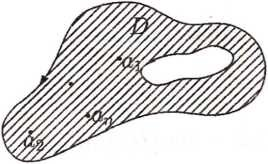
\includegraphics[width=4cm]{Zurag/23.jpg}
    \captionof{figure}{}
        \label{}
\end{center}
байвал 
\begin{eqnarray} \label{6.25}
\int\limits_{\partial D}f(z)dz=2\pi i\sum_{k=1}^n Res [f(z), a_k]
\end{eqnarray} байна.
 \end{thm}
 \begin{prf}
 $a_k(k=\overline{1,n})$ цэгүүд дээр төвтэй хүрэлцээтэй бага $\rho$ радиустай сөрөг чиг барьсан $\gamma_k:|z-a_k|=\rho$ тойргууд татъя. Мөн $|z-a_k|\leq \rho$ дугуйнууд $D$-д агуулагдаж, $\gamma_k$ тойрог бүхэн бусад тойргийнхоо гадна оршин байвал олон холбоост мужийн Кошийн теорем ёсоор
 $$\oint\limits_{\partial D} f(z)dz+\sum_{k=1}^n \oint\limits_{\gamma_k}f(z)dz=0$$
 болж эндээс 
 $$\oint\limits_{\partial D} f(z)dz=\sum_{k=1}^n \oint\limits_{\gamma_k}f(z)dz=2\pi i\sum_{k=1}^n Res [f(z), a_k] $$ 
  \end{prf}
 Онцгой цэг дээрх үлдэцийг олж чаддаг бол (\ref{6.25}) томьёо ашиглан комплекс интеграл бодох боломж нээгдэнэ.
 \begin{thm}
 $a\in\mathbb{C}$ цэг $f(z)$-ийн тусгаарлагдсан онцгой цэг гэвэл
\begin{eqnarray}
Res [f(z), a]=c_{-1}
\end{eqnarray}
 \end{thm}
 \begin{prf}
 (\ref{6.25}) томьёонд $n=-1$ гэвэл
 $$c_{-1}=\frac{1}{2\pi i}\int\limits_{\Gamma'}f(\zeta) d\zeta=Res [f(z),a] \quad \Gamma':|z-a|=R$$ 
  \end{prf}
 \begin{cor}
 $a$ засагдах онцгой цэг бол
 $$Res[f(z),a]=0$$
 \end{cor}
 \begin{thm}
 $f(z)$-функцийн хувьд $a$ нь $n\geq 1$ эрэмбийн туйл байг. Тэгвэл:
 \begin{eqnarray} \label{6.27}
 Res [f(z),a]=\dfrac{1}{(n-1)!}\lim\limits_{z\rightarrow a}\frac{d^{(n-1)}}{dz^{n-1}}[(z-a)^n\cdot f(z)].
 \end{eqnarray}
 \end{thm}
 \begin{prf}
$a$ цэгийн цоорхойт орчинд Лораны цуваанд $f(z)$ функцийг задалбал
$$f(z)=\frac{c_{-n}}{(z-a)^n}+\cdots +\frac{c_{-1}}{z-a}+\sum\limits_{n=0}^\infty c_n(z-a)^n$$
бөгөөд хоёр талыг $(z-a)^n$-ээр үржүүлж $(n-1)$ удаа дифференциалчилбал
$$\frac{d^{(n-1)}}{dz^{n-1}}[(z-a)^n\cdot f(z)]=(n-1)!c_{-1}+n(n-1)!+2c_0(z-a)+\cdots$$
бөгөөд $z\rightarrow a$ хязгаарт шилжвэл (\ref{6.27}) гарна.

$z=a$ нь $f(z)$ функцийн энгийн туйл байхад (\ref{6.27}) томьёо ёсоор ($0!=1$  гэж үзэх тул)
$$Res [f(z),a]=\lim\limits_{z\rightarrow a}(z-a)f(z)$$
юм. Хэрэв $f(z)=\dfrac{\varphi (z)}{\psi(z)}$, $(\varphi, \psi\in H(a)$, $\varphi(a)\neq 0$, $\psi(a)=0)$ бол 
$$Res[f(z),a]=\lim\limits_{z\rightarrow a}f(z)(z-a)=\lim\limits_{z\rightarrow a}\frac{\varphi (z)}{\frac{\psi(z)-\psi (a)}{z-a}}=\frac{\varphi(a)}{\psi '(a)}$$ 
  \end{prf}
 \begin{exm}
 $\tan z$ функцийн $\dfrac{\pi}{2}$ дээрх үлдэц ол.
 \end{exm}
 \begin{sol}
 $\tan z=\dfrac{\sin z}{\cos z}$, $\sin\dfrac{\pi}{2}=1$, $\cos\dfrac{\pi}{2}=0$ тул $$Res \left[\tan z, \dfrac{\pi}{2}\right] =-\sin \frac{\pi}{2}=-1$$
 \end{sol}
 \begin{exm}
 $(z-1)\cdot \sin\dfrac{1}{z-1}$ функцийн $z=1$ дээрх үлдэц ол.
  \end{exm}
\begin{sol}
	(\ref{5.19}) томьёонд $z$-ийн оронд $\dfrac{1}{z-1}$тавибал
	$$\sin\frac{1}{z-1}=\sum\limits_{n=0}^\infty (-1)^n \frac{1}{(2n+1)!(z-1)^{2n+1}}$$ тул 
	$$Res\left[(z-1)\cdot \sin \frac{1}{z-1}, 1\right] =-\frac{1}{6}$$
\end{sol}
\begin{exm}
$\dfrac{\sin 2z}{(z+1)^3}$ функцийн $z=-1$ дээрх үлдэц ол.
\end{exm}
\begin{sol}
    $z=-1$ нь III эрэмбийн туйл тул 
    $$Res \left[\frac{\sin 2z}{(z+1)^3}, -1\right]=\lim\limits_{z\rightarrow -1}\frac{1}{2!}(\sin 2z)''=2\sin 2$$
\end{sol}
\textbf{Төгсгөлгүй алсын цэг дээр үлдэц ямар байх вэ? } 
\begin{dfn}
$$\frac{1}{2\pi i}\int\limits_{\gamma_R}-f(z)dz$$
хэмжигдэхүүнийг $f(z)$ функцийн $\infty$ дээрх үлдэц гэнэ. Үүнд $\gamma^-_R$ нь сөрөг чиг барьсан (нар зөв тойрох) хүрэлцээтэй их радиустай $|z|=R$ тойрог. $f(z)$ функцийг $\infty$-ийн цоорхойт \\ $R<|z|<\infty$ орчинд задалбал
$$f(z)=\sum\limits_{n=-\infty}^\infty c_n z^n$$
бөгөөд $\gamma^-_R$тойргоор гишүүнчлэн интегралчилж, зэрэгтийн ортогональ чанар ашиглавал
$$Res [f(z),\infty]=-c_{-1}$$
\end{dfn}
\begin{thm}
\textbf{(Үлдэцүүдийн бүтэн нийлбэр)} \index{Үлдэцүүдийн бүтэн нийлбэр} $f(z)$ нь $\mathbb{C}$ дээр $a_k(k=\overline{1,n})$ онцгой цэгтэй байвал
\begin{eqnarray}
\sum\limits_{k=1}^nRes [f(z),a_k]+Res [f(z),\infty]=0
\end{eqnarray} байна. 

Энэ хялбар теоремыг өөрөө батална уу.
\end{thm}
\begin{exm}
$\dfrac{e^z}{z^2(z^2+9)}$ функцийн бүх онцгой цэг болон төгсгөлгүй алсын цэг\index{Төгсгөлгүй алсын цэг дээрх үлдэц} дээрх үлдэц ол.
\end{exm}
\begin{prf}
$z=0$ II эрэмбийн туйл,$z=\pm 3i$ энгийн туйлууд.
\begin{align*}
    Res \left[\frac{e^z}{z^2(z^2\pm 9)}, 0\right] &=\frac{1}{2!}\lim\limits_{z\rightarrow 0}\left(\frac{e^z}{z^2+9}\right)'\\
    &=\lim\limits_{z\rightarrow 0} \frac{e^z(z^2+9)-2ze^z}{(z^2+9)^2}=\frac{1}{18};
\end{align*}
\begin{align*}
    &Res \left[\frac{e^z}{z^2(z^2+ 9)}, 3i\right]=\lim\limits_{z\rightarrow 3i}\frac{e^z}{z^2(z+3i)}=-\frac{1}{54}(\sin 3-i\cos 3)\\
   &Res \left[\frac{e^z}{z^2(z^2+ 9)}, -3i\right]=\lim\limits_{z\rightarrow -3i}\frac{e^z}{z^2(z-3i)}=-\frac{1}{54}(\sin 3+i\cos 3)\\
   &Res \left[\frac{e^z}{z^2(z^2+ 9)}, \infty\right]=\frac{1}{27}(\sin 3-3)
\end{align*}
 \end{prf}
\begin{exm}
$\bint\limits_{|z|=1} \dfrac{e^zdz}{z^2(z^2-9)}$ бод. 
\end{exm}
\begin{sol}
    $|z|=1$ тойрог дотор $z=0$ гэсэн II эрэмбийн туйл байх тул
    \begin{align*}
        \bint\limits_{|z|=1} \dfrac{e^zdz}{z^2(z^2-9)}&=2 \pi i Res\left[ \dfrac{e^zdz}{z^2(z^2-9)}, 0\right]\\
        &=2 \pi i \lim\limits_{z\rightarrow 0}\left(\frac{e^z}{z^2-9}\right)'=2\pi i \lim\limits_{z\rightarrow 0}
        \frac{e^z(z^2-9)-2ze^z}{(z^2-9)^2} \\
        &=-\frac{2\pi i}{9}
    \end{align*}
    (үлдэцийн үндсэн теорем ашиглав). 
\end{sol}
\section{Интеграл бодоход үлдэц ашиглах нь}
\begin{enumerate}
    \item [\textbf{I.}] $\bint\limits_0^{2\pi} R(\cos t,\sin t)dt$, $R(u,v)$ нь бодит $u,v$ гэсэн хоёр хувьсагчийн рациональ функц.
    
    
$R(\cos t, \sin t)$ нь $0\leq t\leq 2\pi$ завсар дээр тасралтгүй функц.
Эйлерийн томьёо ёсоор
$$\cos t=\frac{e^{it}+e^{-it}}{2}, \sin t=\frac{e^{it}-e^{-it}}{2}$$
бөгөөд $z=e^{it}$ гэвэл $|z|=1$, $t\in[0,2\pi]$ үед $z=e^{it}$ цэг $z=1$ цэгээс нар буруу (цагийн зүүний эсрэг) чиглэлээр нэгж тойргийг нэг удаа тойрно. $\cos t=\dfrac{z+z^{-1}}{2}$, $\sin t=\dfrac{z-z^{-1}}{2i}$, $dt=\dfrac{dz}{iz}$ байх тул 
\begin{eqnarray}
\begin{split}
    \int\limits_0^{2\pi}R(\cos t,\sin t)dt&=\oint\limits_{|z|=1}R\left(\frac{1}{2}\left[z+\frac{1}{z}\right], \frac{1}{2}\left[z-\frac{1}{z}\right]\right)\frac{dz}{iz} \\
    &=\oint\limits_{|z|=1} \tilde{R}(z)dz,
\end{split}
\end{eqnarray}
$\tilde{R}(z)$ нь рациональ функцүүдийн композиц тул рациональ функц байна. Энэ л функц нь $|z|=1$ дээр голоморф, түүний дотор төгсгөлтэй тооны онцгой цэгтэй учир үлдэцийн онолоор бодогдоно.
\begin{exm}
$\bint\limits_{0}^{2\pi} \dfrac{dt}{\cos t-2}$ бодож гарга.
\end{exm}
\begin{sol}
$$\int\limits_{0}^{2\pi} \dfrac{dt}{\cos t-2} =\int\limits_{|z|=1} \dfrac{dz}{iz\left(\frac{z+z^{-1}}{2}-2\right)}=\frac{2}{i}\oint\limits_{|z|=1}\frac{dz}{z^2-4z+1}$$ болж $\dfrac{2}{i}\dfrac{1}{z^2-4z+1}$ функцийн зөвхөн $z_1=2-\sqrt{3}$ цэг нь $|z|<1$-д орших тул 
\begin{align*}
    \int\limits_{0}^{2\pi} \dfrac{dt}{\cos t-2}& =2\pi i Res\left[ \dfrac{1}{z^2-4z+1}, 2-\sqrt{3}\right] \\
    &=4 \pi \frac{1}{2(2-\sqrt{3})-4} \\
    &=-\frac{2\pi}{\sqrt{3}}
\end{align*}

\end{sol}
\item[\textbf{II.}]
$\bint \limits_{-\infty}^\infty R(x)dx$, $R(x)$ нь бодит тэнхлэг дээр туйл үгүй рациональ функц, $R(x)=\dfrac{P_m(x)}{Q_n(x)}$ гэвэл $P_m(x)$, $Q_n(x)$ олон гишүүнтүүд ба $m+2\leq n$. Өөрөөр хэлбэл $z=\infty $ нь уул $R(x)$ функцийн 2-оос доошгүй эрэмбийн тэг байг.

Бодит тэнхлэгийн $[-R;R]$ хэрчим $|z|=R$, $\im z>0$ хагас тойргоор битүүрэхдээ $R(z)$ функц комплекс хавтгайд орших бүх туйлыг хамран авахаар радиус $R$-ыг сонгон авна.
\begin{center}
    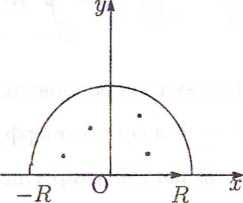
\includegraphics[width=4cm]{Zurag/24.jpg}
    \captionof{figure}{}
        \label{}
\end{center}
$\infty$-ийн орчинд $R(x)$ функцийн Лораны цуваанд задалбал 
$R(z)=\dfrac{c_{-2}}{z^2}+\dfrac{c_{-3}}{z^3}+\cdots$. Иймд $\lim\limits_{z\rightarrow \infty} R(z)\cdot z^2=c_{-2} \ \text{ба} \ \lim\limits_{z\rightarrow \infty}|R(z)|=0,$
$|z|\rightarrow \infty$ үед $|R(z)|\cdot |z|=0(|z|).$ Эндээс аливаа $\varepsilon >0$ тооны хувьд хүрэлцээт их $R$-утганд $\left|\bint\limits_{|z|=R}R(z)dz\right|\leq \varepsilon$. Иймд $R\rightarrow \infty$ үед $\lim\limits_{R\rightarrow \infty}\bint\limits_{|z|=R}R(z)dz=0$ болж улмаар
\begin{eqnarray} \label{6.30}
\begin{split}
    \int\limits_{-\infty}^\infty R(x)dx&= \lim\limits_{R\rightarrow \infty} \int\limits_{-R}^R R(x)dx \\
    &=2\pi i\sum\limits_{k=1}^n Res [R(z), a_k]
\end{split}
\end{eqnarray}
\begin{exm}
$f(z)=\dfrac{1}{(z^2+1)^2}$ функц дээд хагас хавтгайд цор ганц $z=i$ гэсэн II эрэмбийн туйлтай, бодит тэнхлэг дээр туйлгүй бөгөөд $\infty$ нь IV эрэмбийн тэг байх тул (\ref{6.30}) ёсоор 
$$\int\limits_{-\infty}^\infty \frac{dz}{(z^2+1)^2}=2\pi i Res \left[\frac{1}{(z^2+1)^2}, i\right]$$
гэж бодогдоно.

Харин
$$Res \left[\frac{1}{(z^2+1)^2}, i\right]=\lim\limits_{z\rightarrow i} \left[\frac{(z-i)^2}{(z-i)^2(z+i)^2}\right]'=\frac{1}{4i}$$
тул 
$$\int\limits_{-\infty}^\infty \frac{dx}{(x^2+1)^2}=\frac{\pi}{2}.$$
\end{exm}
\item[III.]\textbf{Жорданы лемм.} \index{Жорданы лемм} \\
$F(z)=e^{\lambda iz}\cdot f(z)$, $\lambda>0$, $f(z)$ функц дараах 3 нөхцөлийг хангадаг байг.
\begin{enumerate}
    \item Дээд хагас хавтгайд төгсгөлтэй $n$-тооны онцгой \\ $a_k(k=\overline{1,n})$ цэгтэй,
    \item $Ox$ тэнхлэг дээр төгсгөлтэй $m$-тооны зөвхөн энгийн $x_j(j=\overline{ 1,m})$ туйлтай, 
    \item $\im z \geq 0$ байхаар $z\rightarrow \infty$ үед $f(z)\rightarrow 0$ байвал
\begin{align*}
    \int\limits_{-\infty}^\infty e^{\lambda ix}f(x)dx&= 2\pi i\left\{\sum\limits_{k=1}^n Res[F(z),a_k]+\right.\\
    &\left.+\frac{1}{2}\sum\limits_{j=1}^m Res[F(z), x_j]\right\}
\end{align*}
\end{enumerate}
\begin{center}
    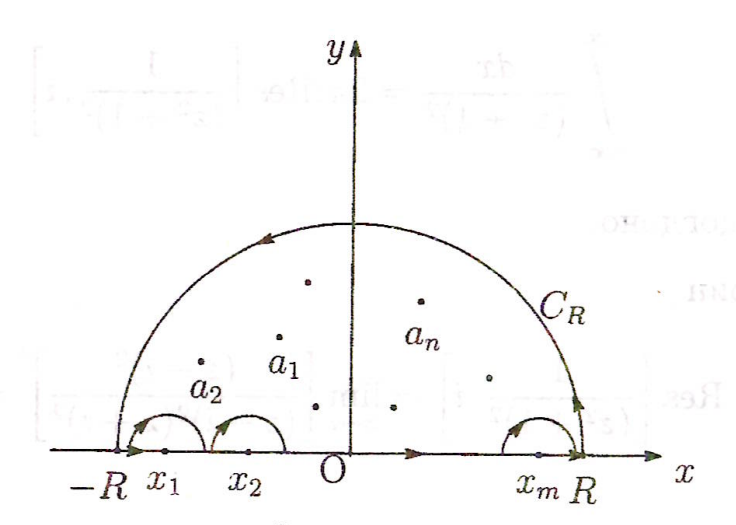
\includegraphics[width=6cm]{Zurag/25.PNG}
    \captionof{figure}{}
        \label{}
\end{center}
\end{enumerate}
\begin{prf}
Бүх $a_k(k=\overline{1,n})$ ба $x_j(j=\overline{1,m})$ онцгой цэгүүдийг хүрээндээ хамрахуйц $C_R:|z|=R$, $\im z>0$ гэсэн хагас тойрог татъя.

Мөн $x_j(j=\overline{1,m})$ цэгүүдэд төвтэй дээд хагас хавтгайд орших, зэргэлдээ хоёр нь ерөнхий цэггүй байхаар $\gamma^-_\rho: |z-x_j|=\rho$, $\im z>0(j=\overline{1,m})$ гэсэн сөрөг тойролттой хагас тойрог авбал үлдэцийн үндсэн теорем ёсоор 
\begin{equation}
    \tag{$*$} \label{*}
    \begin{split}
        &\int\limits_{-R}^{x_1-\rho}F(z)dz+\int\limits_{x_1+\rho}^{x_2-\rho}F(z)dz+\cdots +\\
        &+\int\limits_{x_m+\rho}^RF(z)dz+\sum\limits_{j=1}^m \int\limits_{\gamma_\rho^-}e^{\lambda i z}f(z)dz+\int\limits_{C_R}e^{\lambda iz}f(z)dz = \\
        &=2\pi i\sum\limits_{k=1}^n Res[e^{\lambda iz} f(z), a_k]
    \end{split} 
\end{equation} бөгөөд 
\begin{align*}
    &\lim\limits_{\tiny{\begin{array}{c}
R\to\infty  \\
 \rho\to 0 
\end{array}}}  \left(\int\limits_{-R}^{x_1-\rho} F(z)dz+\cdots +\int\limits_{x_m+\rho}^R F(z)dz\right)=\int\limits_{-\infty}^\infty F(x)dx, \\
    &\lim\limits_{\tiny{\begin{array}{c}
R\to\infty  \\
 \rho\to 0 
\end{array}}}\sum\limits_{j=1}\int\limits_{\gamma^-_\rho}F(z)dz=-\pi i\sum\limits_{j=1}^m Res[F(z), x_j]
\end{align*}
байхыг тооцож хязгаарт шилжсэний дараа (\ref{*}) нь 
\begin{align*}
    &\int\limits_{-\infty}^\infty e^{\lambda ix}f(x)dx+\lim\limits_{\tiny{\begin{array}{c}
R\to\infty  \\
 \rho\to 0 
\end{array}}} \int\limits_{C_R} e^{\lambda iz}f(z)dz= \\
    &=2\pi i\left\{\sum\limits_{k=1}^n Res[F(z), a_k]+\frac{1}{2}\sum\limits_{j=1}^m Res [F(z), x_j]\right\}
\end{align*}
болно. $C_R:z=R(\cos \varphi +i\sin\varphi)$, $0\leq \varphi \leq \pi$ байх тул 
\begin{align*}
    |I_R|&=\left|\int\limits_{C_R}e^{\lambda iz}f(z)dz\right| \\ &=\left|\int\limits_0^\pi e^{\lambda i R\cos \varphi}\cdot e^{-\lambda R\sin \varphi}\cdot f(Re^{i\varphi})\cdot Rid\varphi\right|.
\end{align*}
Гуравдугаар нөхцөл ёсоор $\max\limits_{0\leq \varphi \leq \pi}|f(\re^{i\varphi})|=\sigma(R)\rightarrow 0 (R\rightarrow \infty)$ ба  $|e^{\lambda iR\cos \varphi}|=1$ учир 
$$|I_R|\leq \sigma (R)\int\limits_0 e^{-\lambda R\sin \varphi}d\varphi $$
улмаар хялбар $\sin \varphi >\dfrac{2\varphi}{\pi} \left(\forall \varphi \in\left[0;\dfrac{\pi}{2}\right]\right)$ тэнцэл биш ашиглавал 
$$|I_R|\leq \sigma (R)\int\limits_0^{\frac{\pi}{2}}Re^{-\lambda R\cdot\frac{2\varphi}{\pi}}d\varphi=\frac{\pi \sigma(R)}{\lambda}(1-e^{-\lambda R})\rightarrow 0 (R\rightarrow \infty)$$ 
болж (\ref{*}) тэнцэл:
\begin{eqnarray}\label{6.31}
\begin{split}
    \int\limits_{-\infty}^\infty e^{\lambda ix}f(x)dx& =2\pi i \left\{\sum\limits_{k=1}^nRes[e^{\lambda iz}f(z),a_k]+\right.\\
    &\left.+\frac{1}{2}\sum\limits_{j=1}^m Res[e^{\lambda iz}f(z), x_j]\right\}
\end{split}
\end{eqnarray} 
\begin{exm}
$\int\limits_{0}^\infty \dfrac{\sin ax}{x(x^2+b^2)}dx, \quad (a,b$-эерэг тоонууд) интегралыг бод. 
\end{exm}
 \end{prf}
\begin{sol}
Интеграл доорх функц тэгш, нөгөө талаар \\ $\sin ax=\im e^{iax}$ тул (\ref{6.31}) ёсоор 
\begin{align*}
    \int\limits_0^\infty \frac{\sin ax}{x(x^2+b^2)}dx&=\im \left\{\frac{1}{2}\int\limits_{-\infty}^\infty \frac{e^{iax}}{x(x^2+b^2)}dx\right\} \\
    &=\im \left\{\pi i\left(Res\left[\frac{e^{iaz}}{z(z^2+b^2)}, bi\right]\right.\right.+\\
    &\left.\left.+\frac{1}{2}Res \left[\frac{e^{iaz}}{z(z^2+b^2)},0\right]\right)\right\}
\end{align*} бөгөөд үлдэцүүдийг жич олбол:
$$Res\left[\frac{e^{iaz}}{z(z^2+b^2)}, bi\right] =\lim\limits_{z\rightarrow bi}\frac{e^{iaz}}{z(z+bi)}=-\frac{e^{-ab}}{2b^2}$$
$$Res\left[\frac{e^{iaz}}{z(z^2+b^2)}, 0\right] =\lim\limits_{z\rightarrow 0}\frac{e^{iaz}}{z^2+b^2}=\frac{1}{b^2}$$ болж 
$$\int\limits_0^\infty \frac{\sin ax dx}{x(x^2+b^2)}=\im\left\{\left(\frac{-e^{-ab}}{2b^2}+\frac{1}{2}\frac{1}{b^2}\right)\cdot \pi i\right\}=\frac{\pi}{2b^2}(1-e^{-ab})$$
\end{sol}
\begin{center}
   \textbf{ Дасгал}
\end{center}
Үлдэц ашиглан дараах интегралуудыг бод.

\begin{enumerate}
\colhoy{
    \item $\bint\limits_{0}^{2\pi} \dfrac{d\varphi}{\cos \varphi +3}$;
    \item $\bint\limits_{0}^{2\pi} \dfrac{dx}{\sin x +2}$;
    \item $\bint\limits_{-\infty}^{\infty} \dfrac{dx}{(x^2+1)(x^2+2)}$;
       \item $\bint\limits_{-\infty}^{\infty} \dfrac{(x-1)dx}{(x^2+1)^2};$ }
       \item $\bint\limits_{-\infty}^{\infty} \dfrac{\cos xdx}{x^4+10x^2+9}$;
       \item $\bint\limits_{0}^{\infty} \dfrac{x\sin  ax dx}{x^2+b^2}, \quad (a>0, b>0)$; \colhoy{
          \item $\bint\limits_{-\infty}^{\infty} \dfrac{x\cos x dx}{x^2-5x+6}$;
            \item $\bint\limits_{-\infty}^{\infty} \dfrac{\sin x dx}{x^3-x^2+4x-4}$}
\end{enumerate}
